\chapter{Übertragungsverfahren}

Heute existieren hunderte verschiedener Übertragungserfahren (Siehe auch \link{Betriebsart}). Hier ein kleiner Ausschnitt davon:

\section{CW}
CW (A1A) steht für \textit{Continuous Wave} und wird im Amateurfunk als Synonym für Morsecode verwendet. Die Informationen werden nicht durch das Signal an sich, sondern durch Rhythmus und Pausen übertragen. Da nur ein Trägersignal verwendet wird, ist die Bandbreite mit etwa 300 Hz relativ gering. So sind DX-Verbindungen auf andere Kontinente bei guten Ausbreitungsbedingungen mit wenigen mW möglich.

Die häufiger verwendeten Zeichen sind kürzer, damit die Übertragung effizienter ausfällt. Daneben existieren viele internationale und lokale Abkürzungen.

\textit{Angabe:} Frequenz

\section{RTTY}
\begin{wrapfigure}{R}{4cm}
%%%%%%%%%%%%%%%%%%%%%%%%%%%%%%%%%%%%%%%%%%%%%%%%%%%%%%%%%%%%%%%%%%%%%%%%%%%%%%%%%%%%%%%
%%% You will need to add \usepackage{wrapfig} to your preamble to use textwrapping %%%
%%%%%%%%%%%%%%%%%%%%%%%%%%%%%%%%%%%%%%%%%%%%%%%%%%%%%%%%%%%%%%%%%%%%%%%%%%%%%%%%%%%%%%%
 \centering
 
\includegraphics[height=4cm]{png/RTTY-BaudlineSmall.png}
 % RTTY-BaudlineSmall.png: 47x163 pixel, 72dpi, 1.66x5.75 cm, bb=0 0 47 163
 \caption{RTTY-Wasserfall}
 \label{fig:rttyWaterfall}
\end{wrapfigure}

Radio Teletype war vor PSK31 das am meisten verwendete digitale Übertragungsverfahren unter Amateurfunkern, da sie einfach zu Übermitteln und zu decodieren ist. Ein durch \link{FSK} bzw. AFSK bedingter Nachteil ist die Bandbreite von mehreren 100 Hz: Sie benötigt mehr Leistung und belegt einen grösseren Teil des Frequenzbandes als andere digitale Verfahren. Die Zeichen werden mit dem Baudot-Code codiert. Er wurde von Èmile Baudot für ein Telegrafengerät entwickelt, das mit fünf Fingern bedient werden kann. Einzelne Zeichen haben immer eine Länge von 5 Bit, womit 32 verschiedene Zeichen möglich sind. Da dies für das Alphabet zu wenige sind, wird ein Umschaltcode verwendet, der zwischen der Buchstaben- und der Zahlentabelle wechselt. Geht dieser bei der Übertragung verloren, werden falsche Zeichen angezeigt. Es ist ausserdem möglich, mit invertierter Polarisation zu senden, dann sind Mark und Space vertauscht.

Im Amateurfunk verwendet man standardmässig eine Baudrate von 45.45 Bd und kleinen Shifts von etwa 180 Hz. Der Deutsche Wetterdienst sendet mit 50 Bd.

\textit{Angaben:} Mittelfrequenz, Shift, Baudrate, Polarisation

\subsection{PSK31}
Dieses digitale Übertragungsverfahren existiert erst seit wenigen Jahren. Es wurde von Peter Martinez, g3plx, für den Amateurfunk entwickelt. Anders als andere moderne Übertragungsverfahren soll es keine fehlerfreie Übertragung garantieren, da man mit solchen Verfahren bei schlechten Verbindungsverhältnissen statt nur bruchstückhaftem Text schnell gar nichts mehr empfangen kann. In dieser Hinsicht ist ist PSK31 gut mit CW vergleichbar, da auch mit schwierigen Verhältnissen noch Verbindungen zustande gebracht werden können. Mit 50 wpm entspricht die Übertragungsgeschwindigkeit der durchschnittlichen Anschlagsrate bei der Tastatur.

Durch die sehr geringe Bandbreite (etwa 32 Hz, weniger als CW!), die der Übertragungsrate von 31.25 Bits/s entspricht, kann mit kleiner Leistung über weite Distanzen gesendet werden. Ermöglicht wird dies durch die Phasenmodulation.

\begin{figure}[h!]
 \centering
 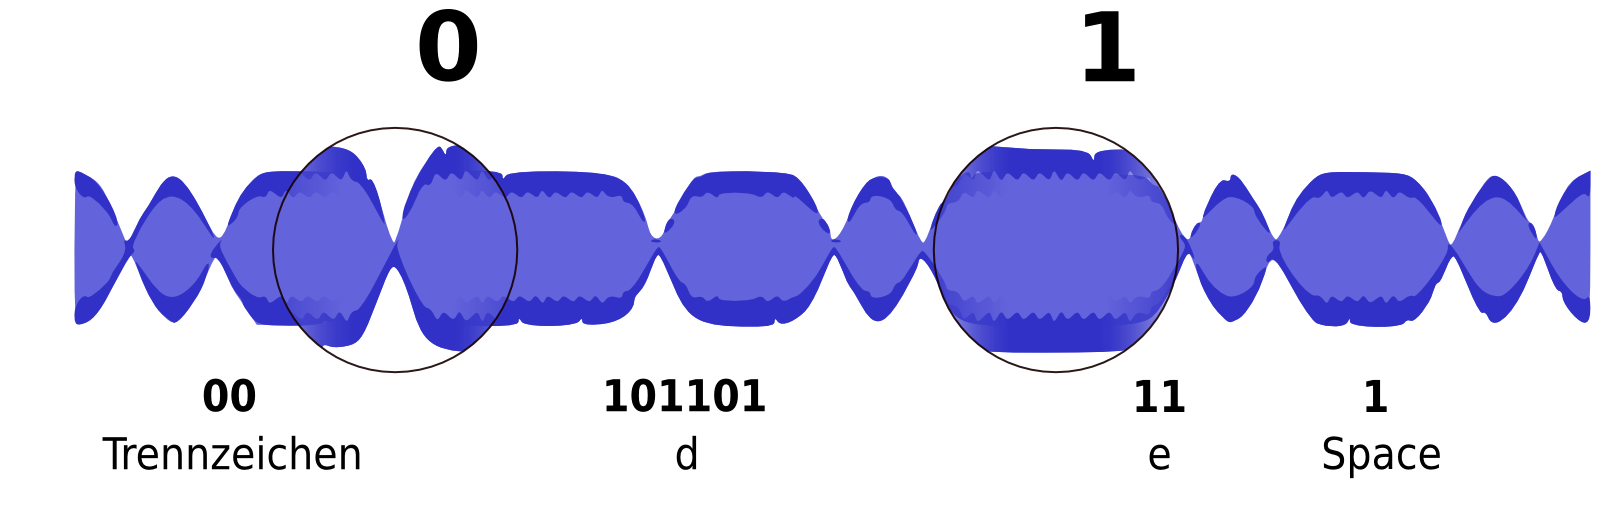
\includegraphics[width=6cm]{./png/Amfu-PSK31-0101.png}
 \caption{Ausschnitt eines PSK31-Datenstroms}
 \label{fig:psk31}
\end{figure}


Die Zeichen werden in Varicode, einer weiteren Entwicklung von g3plx, übermittelt. Sie haben, je nach Häufigkeit (in englischem Text), eine unterschiedliche Länge. Ein Wechsel zwischen zwei Phasen steht für eine 0, eine gleichbleibende Phase für eine 1. Zwei aufeinander folgende Nullen werden als Trennzeichen zwischen zwei Zeichen verwendet.

In der \link{Grafik 13 unten} wird der Text «de» mit PSK31 übermittelt. Das d wird durch 101101 codiert, das e durch 11. Die folgende 1 ergibt einen Leerschlag.

Die Weiterentwicklung QPSK31 ermöglicht mit Quadratur-Phasenmodulation eine schnellere Übertragung. Das Signal wird dabei um ein Vielfaches von 90 Grad verschoben, was vier mögliche Zustände ergibt. 

\textit{Angabe:} Frequenz

\subsection{Olivia}
Ein neueres MFSK-Verfahren. Die Übertragung ist selbst dann noch möglich, wenn das Signal 10 dB unter dem Rauschpegel liegt. Je nach Anzahl Tönen (2 bis 256) beansprucht diese Übertragungsart eine Bandbreite von 125 bis 2000 Hz.

\subsection{Pactor}
Mit PACTOR, einer Weiterentwicklung der digitalen Betriebsart Amtor, ist es möglich, auch bei schlechten Verhältnissen fehlerfrei Daten zu übertragen, da dann zu robusteren Übertragungsverfahren gewechselt wird. Ausserdem kann man auf Mailboxen zugreifen und so mobil Mails abrufen.

Version I überträgt 100--200\,bits/s, PACTOR-IV bis 5512\,bits/s ohne Kompression. Anders als das offene PACTOR sind PACTOR-II und höher allerdings proprietär, das heisst, die genaue Implementierung ist unbekannt, wodurch Modems nur durch den Entwickler SCS hergestellt werden können (und diese deshalb auch entsprechend teurer sind).

Die Daten werden bei PACTOR mittels \link{FSK} übertragen, bei PACTOR-II und höher mit verschiedenen \link{PSK}-Varianten. Bevorzugte Baudraten sind 300 Bd auf HF, 1200 Bd auf VHF/UHF, 9600 Bd auf UHF.

\textit{Angaben:} Frequenz, Baudrate

\subsection{SSTV}
Bei diesem etwas spezielleren computergestützten Verfahren (Slow Scan Television) werden Bilder ausgetauscht. Sie haben üblicherweise 256 Zeilen, dies kann jedoch zwischen den verschiedenen Formaten variieren.

\textit{Angaben:} Frequenz, Format

\subsection{DAB/DRM}
DAB (Digital Audio Broadcasting) und DRM (Digital Radio Mondiale) sind Verfahren zur digitalen Übertragung von Daten (speziell Radiosendungen). Sie basieren beide – wie übrigens auch ADSL – auf OFDM \textit{(Orthogonal Frequency Division Multiplex)}, also der gleichzeitigen Übertragung von mehreren hundert (bei DAB bis 1536) PSK-Strömen. Die Signale sind ungefähr 10 kHz breit bei DRM bzw. etwa 1.5 MHz bei DAB. Neben Ton können über verschiedene Dienste auch andere Daten übertragen werden. Das \textit{MOT} (Multimedia Object Transfer Protocol) etwa ermöglicht die Verteilung von Dateien. So werden parallel zu Radiosendungen komplette Internetseiten mit News übertragen (BWS, Broadcast Webpage System). Per \textit{DLS} (Dynamic Label Service) werden Informationen zur Laufenden Sendung (Name des Stücks, Interpret) übermittelt.

DRM wird auf HF eingesetzt, auf VHF/UHF verwendet man (noch) DAB. DRM+ (DRM für VHF/UHF) hätte hier jedoch einige Vorteile wie bessere Qualität und die Möglichkeit, einzelne Stationen auszusenden; so könnten kleinere Stationen ihre Sendemasten beibehalten.

Nachteilig ist bei Taschenradios der durch die Decodierung bedingte hohe Stromverbrauch.

\subsection{Weitere Übertragungsverfahren}
ATV (Amateur Television), Clover, DATV (Digital Amateur Television), FAX, G-TOR, Hell, JT65, MT63, Packet Radio, SITOR (Simplex Teleprinting Over Radio) 
